\chapter{R\'esultats et discussions}

Apr\`es avoir d\'efini notre approche m\'ethodologique lors de la phase
pr\'ec\'edente, nous allons d\'esormais poursuivre notre \'etude en
nous int\'eressant dans le d\'etail \`a chacun des m\`emes choisis. Les
choix m\'ethodologiques de cette \'etude cherchent notamment \`a
d\'emontrer que les actes de communication ne peuvent simplement se
comprendre comme des \'echanges
{\textquotedblleft}sociaux{\textquotedblright} mais doivent \^etre
appr\'ehend\'es plus largement comme des actes
d{\textquoteright}\'enonciation complexes poss\'edant de multiples
dimensions s\'emantiques, temporelles, conversationnelles toutes
localis\'ees.


\section{R\'esultats}
Nous allons donc maintenant consid\'erer les diff\'erents aspects de
chacun des m\`emes s\'electionn\'es auparavant afin de mieux comprendre
comment diff\'erentes lectures peuvent nous informer sur les
diff\'erents aspects de chacune de leur diffusion.


Pour une meilleure commodit\'e de lecture, un nom a \'et\'e attribu\'e
\`a chacun des m\`emes \'etudi\'es qui permettra de
l{\textquoteright}\'evoquer facilement tout au long du chapitre qui
suit. Une pr\'esentation plus d\'etaill\'ee de chaque m\`eme est
disponible en annexe de cette th\`ese.


\begin{figure}
  \begin{tabular}{c|c}

    \textbf{Nom} &
    \textbf{Description}\\

    \textit{S}\textit{extape}\textit{ } &
    Un scandale d{\textquoteright}adult\`ere concernant un homme politique
    dans la ville de Chongqing dans le centre de la Chine.\\

    \textit{The Voice } &
    La premi\`ere saison d{\textquoteright}une \'emission de
    t\'el\'e-crochet musical en Chine.\\

    \textit{Qiegao } &
    Un d\'ebat de soci\'et\'e sur la condition du peuple Uyghur suivant un
    fait divers autour d{\textquoteright}une rixe lors
    d{\textquoteright}une vente de g\^ateau.\\

    \textit{Dufu} &
    Un m\`eme comique mettant en sc\`ene un po\`ete chinois dans des
    situations burlesques.\\

    \textit{Biaoge} &
    Un scandale entourant la collection de montres de marques prestigieuses
    d{\textquoteright}un homme politique de la province du Shaanxi \\

    \textit{Moyan} &
    L{\textquoteright}attribution du Prix Nobel de litt\'erature \`a
    l{\textquoteright}\'ecrivain chinois Mo Yan\\

    \textit{Yuanfang} &
    La reprise d{\textquoteright}une citation d{\textquoteright}une s\'erie
    t\'el\'evis\'ee sous forme humoristique\\

    \textit{Ccp} &
    D\'ebats entourant le 18\`eme Congr\`es du Parti Communiste Chinois\\

  \end{tabular}
  \caption{D\'enomination et description des m\`emes \'etudi\'es}
\end{figure}


\subsection[Approches socio{}-s\'emantiques et temporelles de la diffusion]{Approches socio-s\'emantiques et temporelles de la diffusion}

\subsubsection[Structures temporelles]{4111 Structures temporelles}
Dans un premier temps, nous avons choisi de consid\'erer les
diff\'erentes structures temporelles des m\`emes. Les figures
ci-dessous repr\'esentent chronologiquement le volume de messages
\'echang\'es par heure dans chacun des jeux de donn\'ees. La dur\'ee
totale des \'echantillons ci-dessous est de 3 semaines. La diminution
r\'eguli\`ere de la quantit\'e de messages observ\'es dans les graphes
correspond \`a la baisse d{\textquoteright}activit\'e pendant les
nuits.

\begin{figure}
    \centering
    \subfloat[]{
      \label{fig:edge-a}
      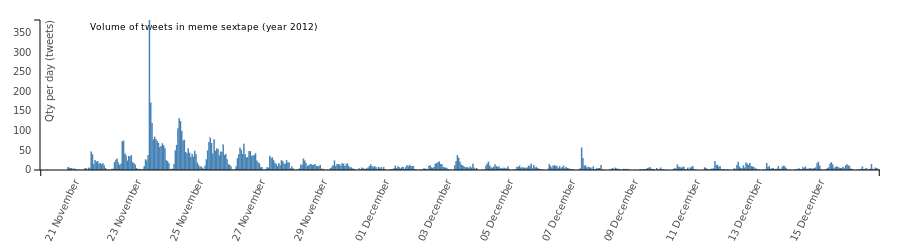
\includegraphics[width=6.0087in,height=1.6697in]{figures/chap4/chapitre4-img1.png}
    }
    \subfloat[]{
      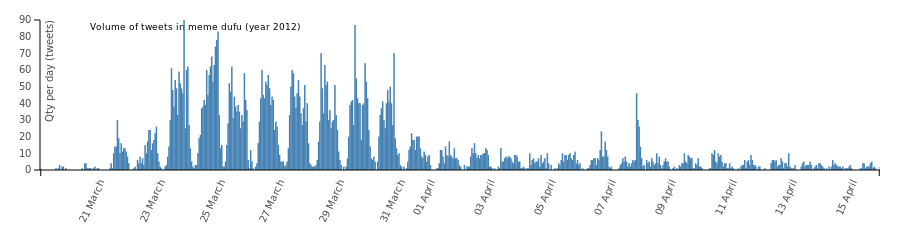
\includegraphics[width=6.0087in,height=1.6697in]{figures/chap4/chapitre4-img2.png}
    }
    \subfloat[]{
      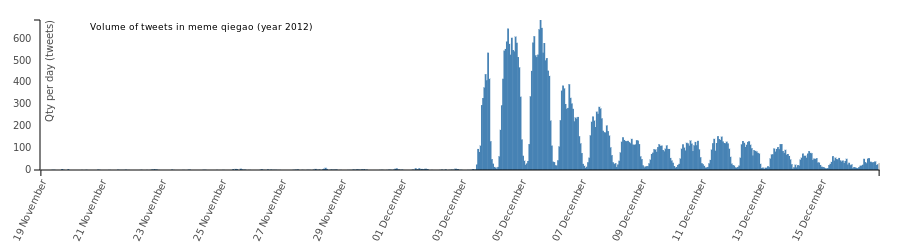
\includegraphics[width=6.0087in,height=1.6697in]{figures/chap4/chapitre4-img3.png}
    }
    \subfloat[]{
      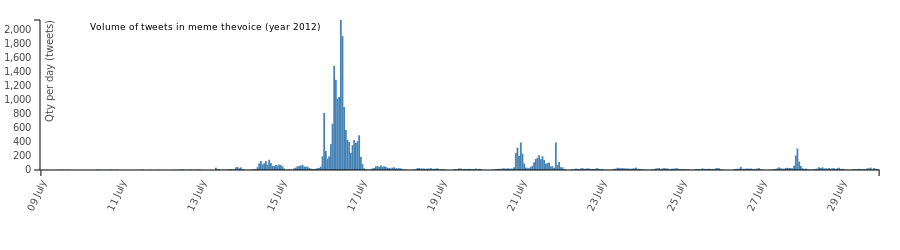
\includegraphics[width=6.0087in,height=1.6697in]{figures/chap4/chapitre4-img4.png}
    }
    \caption{
      Graphe temporel repr\'esentant le volume de messages \'echang\'es sur une dur\'ee de 3 semaines    
    }
\end{figure}


D{\textquoteright}apr\`es ces figures, nous pouvons constater
diff\'erentes formes repr\'esentatives : la {\textquotedblleft}breaking
news{\textquotedblright} du m\`eme \textit{qiegao} se voit nettement
par un d\'epart abrupt de la courbe (fig. F-3) \`a un niveau
directement tr\`es \'elev\'e, suivi d{\textquoteright}une retomb\'ee
rapide de l{\textquoteright}attention en quelques jours . 

La discussion plus informative autour du proc\`es de
l{\textquoteright}homme politique de Chongqing et sa
{\textquotedblleft}sextape{\textquotedblright} (fig. F-1) croit
doucement pour conna\^itre un pic rapide et tr\`es fort de discussion
avant de retomber rapidement \'egalement. 

L{\textquoteright}\'emission de t\'el\'evision The Voice est, elle,
absolument \'ev\`enementielle et son graphe montre bien le rythme des
\'emissions accompagn\'ees de tr\`es peu de discussions entre les
\'emissions (fig. F-2). N\'eanmoins, nous voyons que le volume est
nettement plus important avec un pic de plus de 2000 tweets dans une
m\^eme heure le soir de la premi\`ere \'emission, d\'epassant tr\`es
largement les trois autres m\`emes pr\'esent\'es. 

Le graphe du m\`eme absurdiste
{\textquotedblleft}dufu{\textquotedblright} connait une lente mont\'ee
d{\textquoteright}attention puis un plateau de plusieurs jours. La
blague semble durer et m\^eme conna\^itre un regain
d{\textquoteright}int\'er\^et une semaine plus tard et \^etre
r\'eguli\`erement mentionn\'e par la suite (fig. F-4). 

Proportionnellement, nous constatons que le m\`eme absurdiste est celui
qui retient le plus l{\textquoteright}attention, le plus longtemps
(fig. F-4). A l{\textquoteright}inverse la campagne en ligne de The
Voice n{\textquoteright}est qu{\textquoteright}un artefact de
l{\textquoteright}\'emission (fig. F-2) mais draine une audience tr\`es
importante pendant un temps restreint.


La tendance du m\`eme comique \`a durer se v\'erifie \'egalement avec
\textit{yuanfang }qui continue d{\textquoteright}\^etre mentionn\'e
tr\`es r\'eguli\`erement sur une p\'eriode de plusieurs mois (ici du 7
Octobre au 16 D\'ecembre 2012). 

\begin{figure}
    \centering
    
  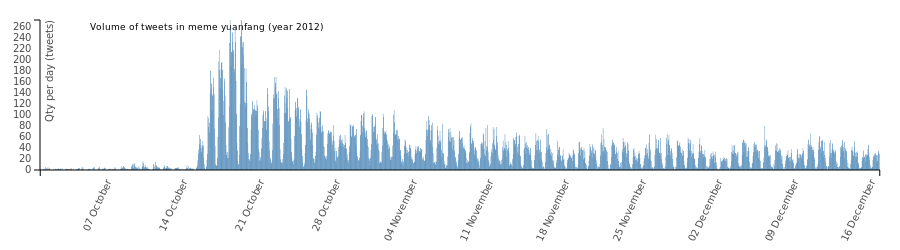
\includegraphics[width=6.0087in,height=1.6697in]{figures/chap4/chapitre4-img5.png}
    
  \caption{
   Graphe temporel repr\'esentant le volume de messages \'echang\'es  autour du m\`eme \textit{yuanfang} entre le 7 Octobre et le 16 D\'ecembre 2012.
  }
\end{figure}


A l{\textquoteright}inverse, les informations type {\textquotedblleft}news{\textquotedblright} ont une dur\'ee de vie tr\`es courte, m\^eme lorsqu{\textquoteright}elles sont tr\`es d\'ebattues. Dans le cas de Moyan, on voit un tr\`es fort volume d{\textquoteright}activit\'e (3000 messages par heure au plus haut) mais une disparition quasi-totale des d\'ebats au bout en moins d{\textquoteright}une dizaine de jours.

\begin{figure}
    \centering
    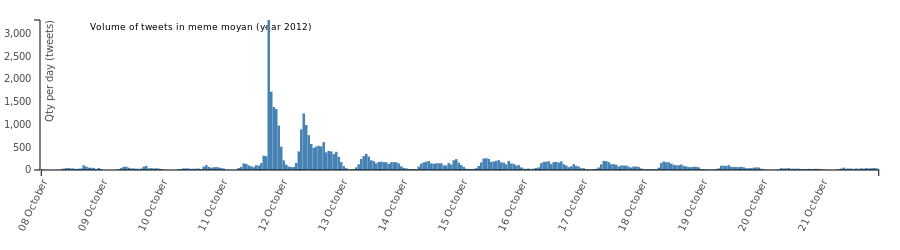
\includegraphics[width=6.0087in,height=1.6697in]{figures/chap4/chapitre4-img6.png}
    \caption{
      Graphe temporel repr\'esentant le volume de messages \'echang\'es autour du m\`eme \textit{moyan} entre le 8 et le 21 Octobre 2012.
    }
\end{figure}

\subsubsection[Structures conversationnelles]{Structures
conversationnelles}
Les conversations sur Sina Weibo sont faites
d{\textquoteright}\'echanges entre les utilisateurs sous la forme de
commentaires, de promotion d{\textquoteright}un message
({\textquotedblleft}chuanfa{\textquotedblright} \'equivalent du
{\textquotedblleft}retweet{\textquotedblright} de Twitter) ou de
r\'eponse au message. Ces diff\'erentes interactions forment dans leur
ensemble une large conversation o\`u les utilisateurs interagissent, se
parlent, se r\'epondent, discutent en utilisant les diff\'erentes
fonctionnalit\'es de la plateforme. En simplifiant ces \'echanges sous
la forme de relation dirig\'ee entre deux utilisateurs
(\textit{{\textquotedblleft}A interagit avec B{\textquotedblright}}),
nous pouvons reconstituer le r\'eseau des interactions que nous
visualisons ensuite sous la forme d{\textquoteright}un graphe. 


Dans notre repr\'esentation, chaque utilisateur est un point et chaque
interaction correspond \`a un trait. La couleur des points montre
l{\textquoteright}appartenance de l{\textquoteright}utilisateur \`a une
m\^eme communaut\'e de conversation calcul\'e gr\^ace \`a un algorithme
de Louvain (Blondel \& al., 2008). La taille des points expriment le
nombre total de connexions entrantes et sortantes d{\textquoteright}un
utilisateur. La distance entre les groupes
d{\textquoteright}utilisateurs est d\'efinie en utilisant
l{\textquoteright}algorithme \textit{force }de d3js (Bostock \& al.,
2011) pour calculer leur r\'epulsion : plus les utilisateurs sont
proches dans la conversation, plus les points les repr\'esentant sont
proches dans le graphe. La forme circulaire du graphe est due aux
propri\'et\'es physiques d{\textquoteright}attraction utilis\'ees lors
du calcul qui permettent aux diff\'erents nodes du graphe de rester
agr\'eger ensemble sans se diss\'eminer. Pour des questions de
lisibilit\'e, seuls les 500 utilisateurs les plus actifs ont \'et\'e
repr\'esent\'es. Les utilisateurs poss\'edant moins de deux
interactions ont \'et\'e supprim\'es pour rendre le graphe lisible.

\begin{figure}
    \centering
    \subfloat[Sextape]{
      \label{fig:edge-a}
      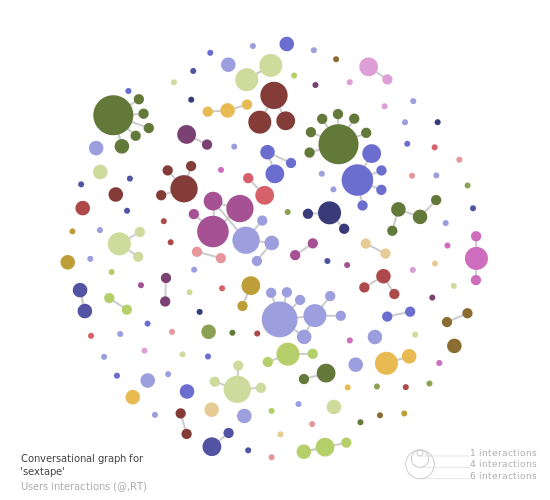
\includegraphics[width=3.0705in,height=2.7913in]{figures/chap4/chapitre4-img7.png}
    }
    \subfloat[The Voice]{
      \label{fig:edge-a}
      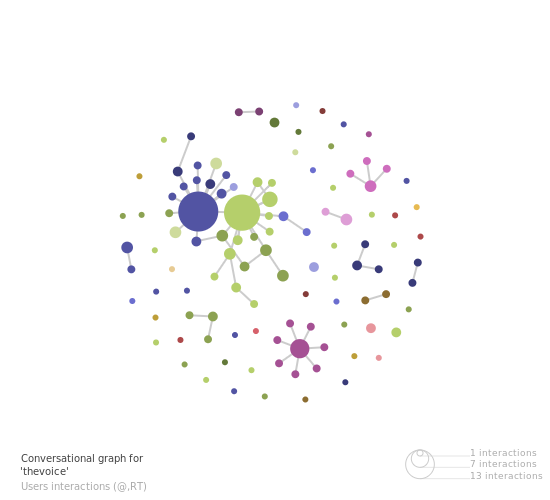
\includegraphics[width=3.0705in,height=2.7913in]{figures/chap4/chapitre4-img8.png}
    }
    \subfloat[Qiegao]{
      \label{fig:edge-a}
      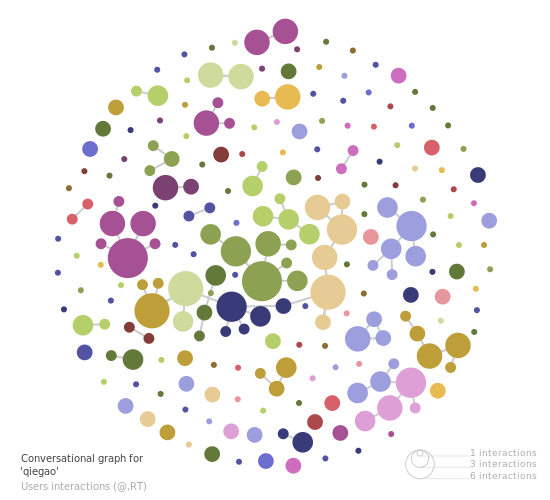
\includegraphics[width=3.0705in,height=2.7913in]{figures/chap4/chapitre4-img9.png}
    }
    \subfloat[Dufu]{
      \label{fig:edge-a}
      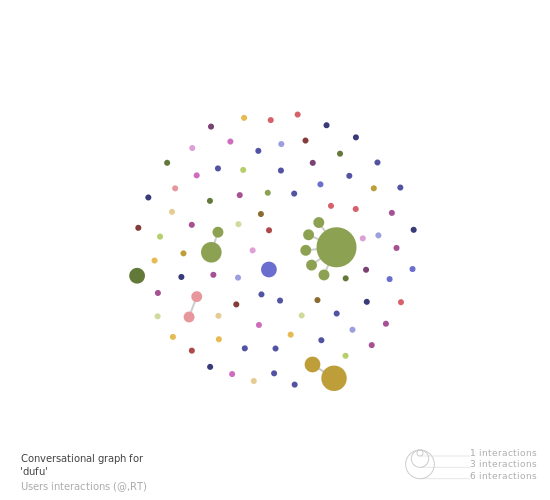
\includegraphics[width=3.0748in,height=2.7953in]{figures/chap4/chapitre4-img10.png}
    }
    
  \caption{  
    Graphe conversationnel pour chacun des 4 m\`emes (pour une dur\'ee de 3 semaines)
  }
\end{figure}

Les graphes de conversation permettent d{\textquoteright}identifier des
sp\'ecificit\'es et de lire plusieurs indicateurs. Ils rendent
notamment bien compte de la taille des conversations, tr\`es variables,
ou plut\^ot de la dimension des interactions. On voit que les
discussions autour d{\textquoteright}aspects politiques et soci\'etaux
connaissent beaucoup plus d{\textquoteright}\'echanges, alors que les
deux autres semblent moins importantes. Dans le cas de \textit{The
Voice} (Fig. H-2), la conversation est tr\`es structur\'ee autour de
peu d{\textquoteright}acteurs qui centralisent les d\'ebats. Le m\`eme
absurdiste \textit{dufu }(fig.H-4) semble \^etre compos\'e
d{\textquoteright}utilisateurs tr\`es distants qui ne communiquent
entre eux que faiblement ou par petits groupes. La conversation
\textit{sextape }autour du fait divers politique se constitue en
groupes structur\'es mais plus distants, repouss\'es vers les bords du
graphe, montrant l{\textquoteright}existence de nombreux foyers de
discussions. A l{\textquoteright}inverse, la discussion de soci\'et\'e
\textit{qiegao}\textit{ }autour des peuples du Xinjiang (fig. H-3)
semble constitu\'e autour d{\textquoteright}un vaste foyer de
discussions o\`u viennent s{\textquoteright}agr\'eger de nombreux
utilisateurs tr\`es actifs.

\subsubsection[Structures s\'emantiques]{Structures s\'emantiques}
La dimension lexicale des contenus web pr\'esente une autre approche
int\'eressante \`a explorer pour mieux comprendre comment se structure
l{\textquoteright}activit\'e lors de la diffusion des m\`emes. La
repr\'esentation classique du nuage de mots
s{\textquoteright}int\'eresse principalement \`a la quantit\'e de mots
en laissant toutefois de cot\'e l{\textquoteright}aspect relationnel de
l{\textquoteright}existence des mots qui est pourtant le fondamental de
l{\textquoteright}activit\'e symbolique et expressive. Ainsi, nous
avons plut\^ot choisi de nous int\'eresser aux r\'eseaux de mots afin
de comprendre comment l{\textquoteright}activit\'e en ligne se
construit autour de signifi\'es particuliers.


Les graphes de mots pr\'esent\'es ici sont construits gr\^ace aux
co-occurences de mots dans les messages. Si deux mots sont utilis\'es
dans un m\^eme message, un \textit{edge} est ajout\'e entre eux,
recr\'eant ainsi un graphe pond\'er\'e repr\'esentant une structure
s\'emantique relationnelle d{\textquoteright}ensemble entre les mots.
La taille des mots repr\'esente le nombre de fois o\`u il sont \'et\'e
cit\'es dans l{\textquoteright}ensemble du corpus. Les couleurs
d\'efinissent des communaut\'es de mots qui ont \'et\'e calcul\'ees
gr\^ace \`a l{\textquoteright}algorithme de Louvain (Blondel \& al.,
2008). L{\textquoteright}\'epaisseur des traits repr\'esentent
l{\textquoteright}intensit\'e des relations (leur nombre de
co-occurences dans le corpus). La disposition des mots utilise
\'egalement l{\textquoteright}algorithme Force de d3js (Bostock \& al.,
2011) pour calculer la proximit\'e des mots sur la base de
l{\textquoteright}intensit\'e de leurs relations. Afin de limiter la
taille du graphe, nous avons s\'electionn\'e uniquement les 500 mots
les plus utilis\'es. 


Un des biais importants \`a prendre en compte dans la lecture de ces
graphes est le fait que les corpus desquels ils sont extraits ont
\'et\'e constitu\'es gr\^ace \`a une recherche par mots-cl\'es dans un
moteur d{\textquoteright}indexation. Ainsi, les mots les plus
pro\'eminents sont ceux qui sont \`a l{\textquoteright}origine de la
constitution du corpus.

\begin{figure}
    \centering
    \subfloat[Dufu]{
      \label{fig:edge-a}
      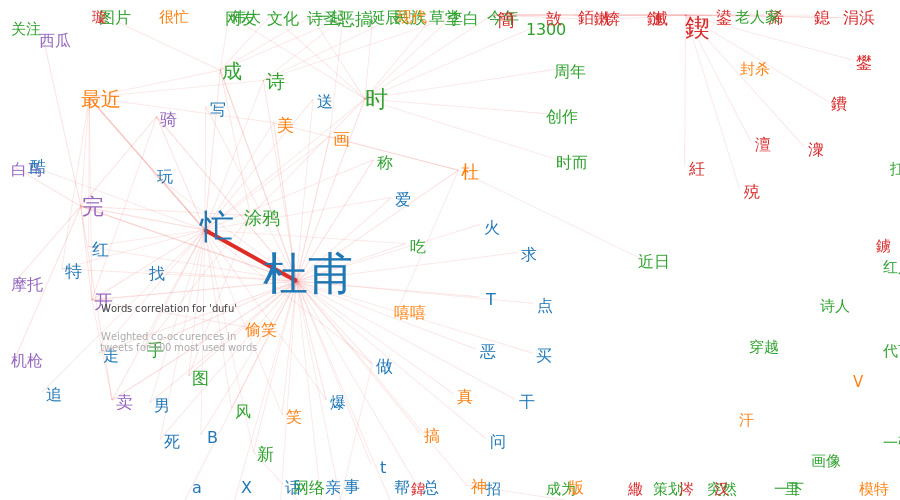
\includegraphics[width=3.1661in,height=1.7594in]{figures/chap4/chapitre4-img11.png}
    }
    \subfloat[Yuanfang]{
      \label{fig:edge-a}
      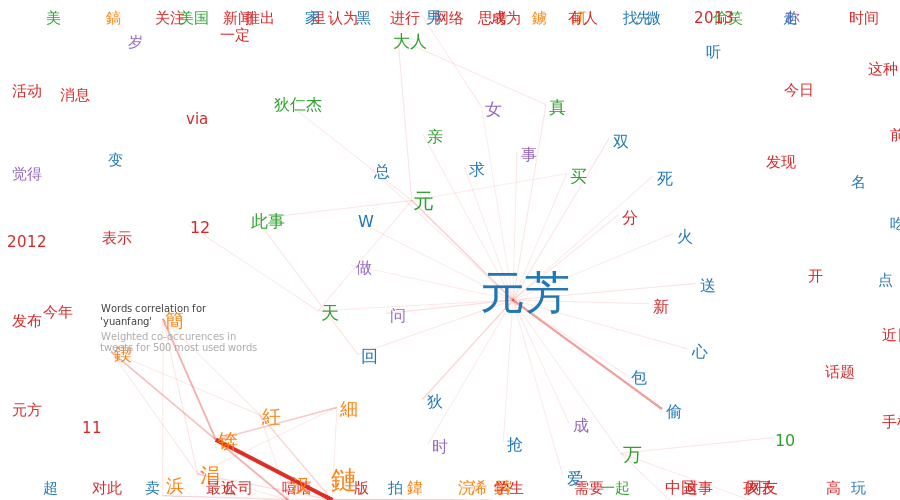
\includegraphics[width=3.1835in,height=1.7697in]{figures/chap4/chapitre4-img12.png}
    }
    
  \caption{
    Graphe s\'emantique de co-occurences des mots pour les m\`emes absurdistes dufu et yuanfang   
  }
\end{figure}
 

En regardant ces graphes, nous constatons tout d{\textquoteright}abord
que les graphe des m\`emes absurdistes se compose de peu de mots
centraux tr\`es fortement connect\'es et entour\'e
d{\textquoteright}une myriade de mots de faible densit\'e,
correspondant s\^urement aux myriades de d\'eclinaisons qui font le
propre de la blague en ligne. 

\begin{figure}
    \centering
    \subfloat[Sextape]{
      \label{fig:edge-a}
      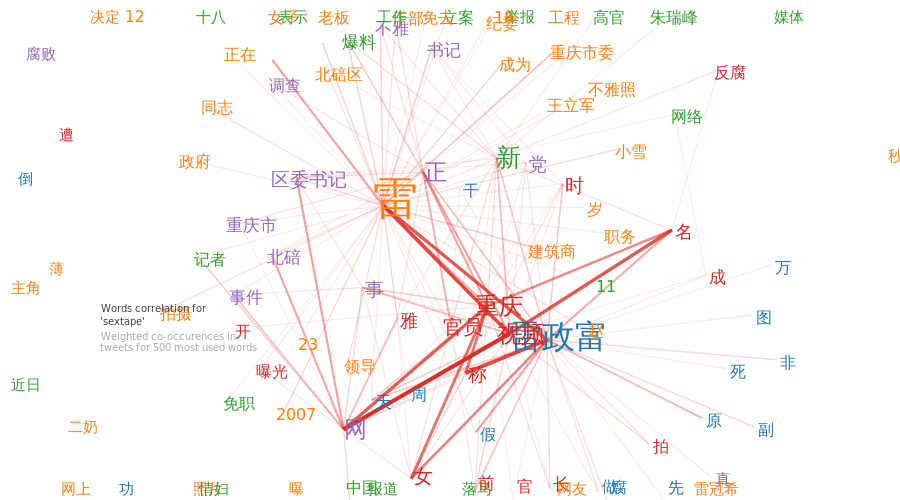
\includegraphics[width=3.1461in,height=1.7504in]{figures/chap4/chapitre4-img13.png}
    }
    \subfloat[biaoge]{
      \label{fig:edge-a}
      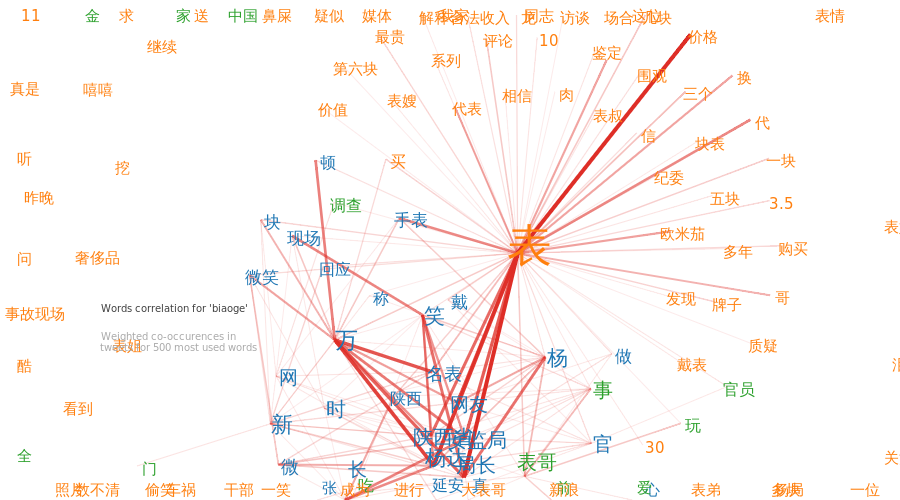
\includegraphics[width=3.2335in,height=1.7961in]{figures/chap4/chapitre4-img14.png}
    }
    
  \caption{
    % Graphe s\'emantique de co-occurences des mots pour les m\`emes absurdistes dufu et yuanfang   
  }
\end{figure}


Les r\'eseaux s\'emantiques de la discussion concernant les faits divers
politiques sont plus structur\'es. Ils sont organis\'es en
communaut\'es de mots et de sens plut\^ot bien d\'efinies : une
communaut\'e d\'ecrit les d\'etails de l{\textquoteright}affaire (noms
de lieux et de personnes, verbes d{\textquoteright}actions),
l{\textquoteright}autre se compose d{\textquoteright}adjectifs
discutant le caract\`ere houleux de ces histoires, la derni\`ere est
faite de mots plus anecdotiques. 

\begin{figure}
    \centering
    \subfloat[ccp]{
      \label{fig:edge-a}
      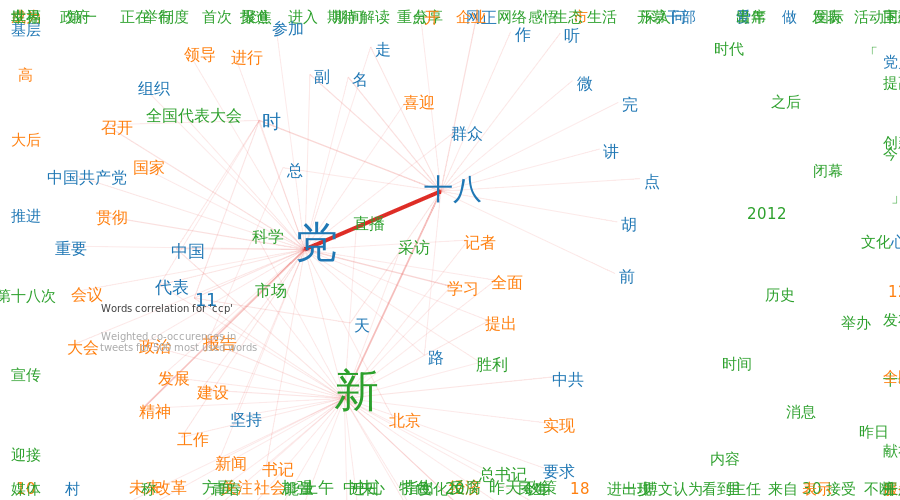
\includegraphics[width=3.0843in,height=1.7134in]{figures/chap4/chapitre4-img15.png}
    }
    \subfloat[The Voice]{
      \label{fig:edge-a}
      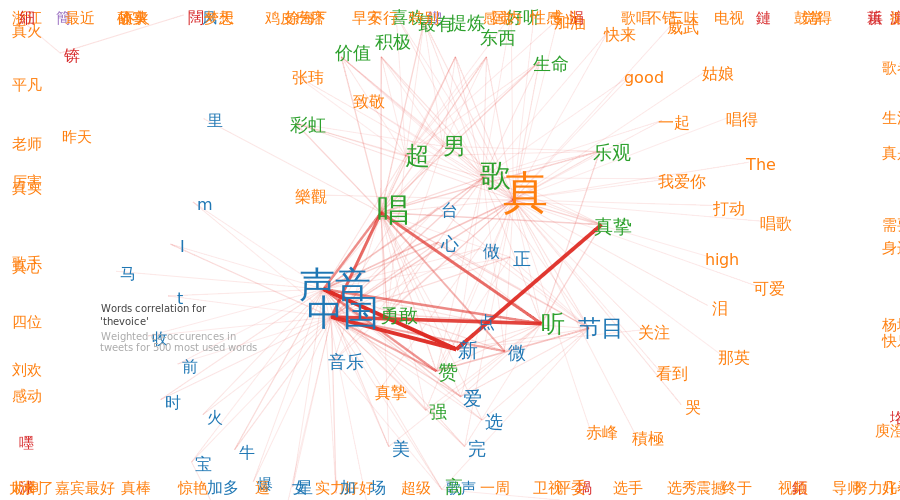
\includegraphics[width=3.0752in,height=1.7122in]{figures/chap4/chapitre4-img16.png}
    }
    
  \caption{
    % Graphe s\'emantique de co-occurences des mots pour les m\`emes absurdistes dufu et yuanfang   
  }
\end{figure}

La structure lexicale qui entoure \textit{The Voice }et \textit{CCP
}semble tr\`es architectur\'ee, avec des associations plus convenues.
Pour \textit{The Voice }(4)\textit{, }nous sommes sans surprise en
pr\'esence du champ lexical du chant (voix-chant, chant-chanson...)
entour\'e par de nombreuses \'emotions et sentiments
(arc-en-ciel-amour, trac-courage, etc.). Nous voyons \'egalement que de
tr\`es nombreux mots ont \'et\'e propuls\'es sur les bords du graphe
car peu reli\'es entre eux ou avec le reste du r\'eseau. Ils sont
d{\textquoteright}ailleurs reconnus algorithmiquement comme une seule
communaut\'e. Il int\'eressant de constater qu{\textquoteright}on y
trouve notamment le vocabulaire propre de l{\textquoteright}\'emission,
qui apparemment ne s{\textquoteright}int\`egre pas aux discussions.
Dans le cas du congr\`es du parti communiste chinois, on retrouve
\'egalement cette organisation s\'emantique tr\`es hi\'erarchique
autour du mot central {\textquotedblleft}parti{\textquotedblright},
avec un ensemble de signifiants issus du programme politique
(construction, d\'eveloppement, loi, science, etc.). Un autre
\'el\'ement pr\'edominent s{\textquoteright}articule autour du
caract\`ere {\textquotedblleft}nouveau{\textquotedblright}
(r\'evolution, changement, futur...). Comme dans le cas de \textit{The
Voice}, nous sommes en pr\'esence d{\textquoteright}un langage
st\'er\'eotyp\'e qui donne lieu \`a un graphe tr\`es structur\'e selon
des axes de communication d\'efinis. Proportionnellement, une grande
partie des discussions est situ\'e aux fronti\`eres du graphe, tr\`es
peu reli\'ee avec le reste de l{\textquoteright}activit\'e.

\begin{figure}
    \centering
    \subfloat[qiegao]{
      \label{fig:edge-a}
      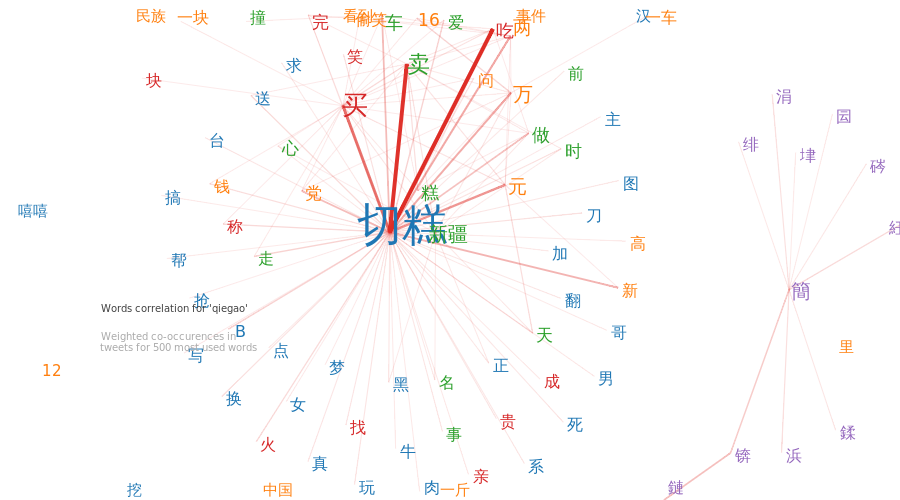
\includegraphics[width=2.9248in,height=1.6252in]{figures/chap4/chapitre4-img17.png}
    }
    \subfloat[moyan]{
      \label{fig:edge-a}
      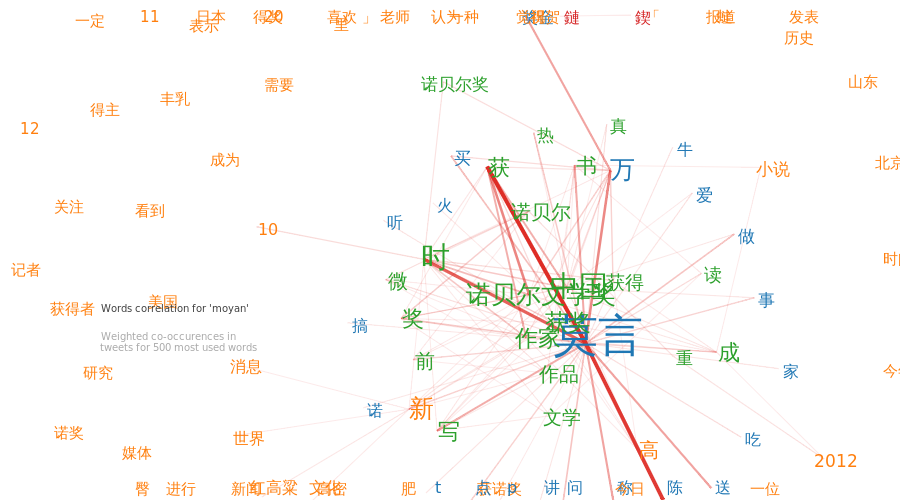
\includegraphics[width=2.978in,height=1.6551in]{figures/chap4/chapitre4-img18}.png 
    }
    
  \caption{
    % Graphe s\'emantique de co-occurences des mots pour les m\`emes absurdistes dufu et yuanfang   
  }
\end{figure}


\textit{Qiegao}, quant \`a lui, poss\`ede une structure tr\`es
centralis\'ee articul\'ee autour d{\textquoteright}un mot-cl\'e
pr\'ecis qui relie plusieurs groupes s\'emantiques (communaut\'es de
mots par couleurs) autour de lui. On retrouve cette caract\'eristique
d{\textquoteright}ensemble dans le graphe de \textit{moyan }m\^eme si
la structuration des communaut\'es s\'emantiques est plus accentu\'ee -
on peut penser que cela est d\^u aux plus grands volumes de messages
\'echang\'es.

\subsection[Structures g\'eographiques et multi{}-graphes]{Structures g\'eographiques et multi-graphes}
Nous avons propos\'e dans cette recherche le terme de milieu num\'erique
afin notamment de probl\'ematiser les rapports existants entre les
pratiques de la discussion en ligne sur Sina Weibo et
l{\textquotesingle}espace de la Chine urbaine moderne. Afin de
poursuivre notre interrogation, nous allons d\'esormais observer
comment les topologies de diffusion en ligne peuvent se corr\'eler avec
la diffusion g\'eographique. La diffusion d{\textquotesingle}un m\`eme
suit-elle la hi\'erarchie urbaine classique ou bien la la g\'eographie
urbaine de l{\textquotesingle}Internet? Existe-t-il des mod\`eles de
diffusion selon les types de contenus? Quels sont les \textit{patterns
}g\'eographiques d\'ecrits pas la circulation des contenus?


Pour tenter de r\'epondre \`a ces diff\'erentes questions, nous
disposons de donn\'ees concernant l{\textquoteright}origine des
utilisateurs, d{\textquoteright}apr\`es les provinces dans leur profil
Sina Weibo. En mettant en relations ces informations de profils avec
les diff\'erentes dimensions d\'efinies pr\'ec\'edemment, nous allons
proc\'eder \`a l{\textquoteright}analyse de la diffusion g\'eographique
des m\`emes.

\subsubsection{ Dynamiques des discussions entre provinces}
Nous avons pr\'ec\'edemment extrait pour chaque m\^eme le r\'eseau
conversationnel des interactions entre utilisateurs. En associant
chaque utilisateur \`a sa province d{\textquoteright}origine, \ nous
pouvons reconstituer le r\'eseau des interactions entre provinces. Afin
d{\textquoteright}observer comment les provinces
s{\textquoteright}associent lors de la discussion, nous pr\'esentons le
r\'eseau des interactions sous la forme d{\textquoteright}une graphe
pond\'er\'e et dirig\'e. Un des biais classique de la cartographie des
r\'eseaux sociaux est de reproduire simplement les foyers de
population. Afin de r\'etablir un \'equilibre est de faire appara\^itre
des dynamiques plus particuli\`eres, les r\'esultats ont \'et\'e
pond\'er\'e par le pourcentage de population totale repr\'esent\'ee par
chaque province dans le corpus utilis\'e (Weiboscope). Pour des raisons
de lisibilit\'e, les liens entre les provinces sont dirig\'es non pas
vers la capitale de la province mais vers le \textit{centroid
(barycentre) }de la forme g\'eom\'etrique qui la repr\'esente.
L{\textquoteright}\'epaisseur des traits exprime le volume
d{\textquoteright}\'echanges en pourcentage du total sur la p\'eriode
observ\'ee.

\begin{figure}
    \centering
    
    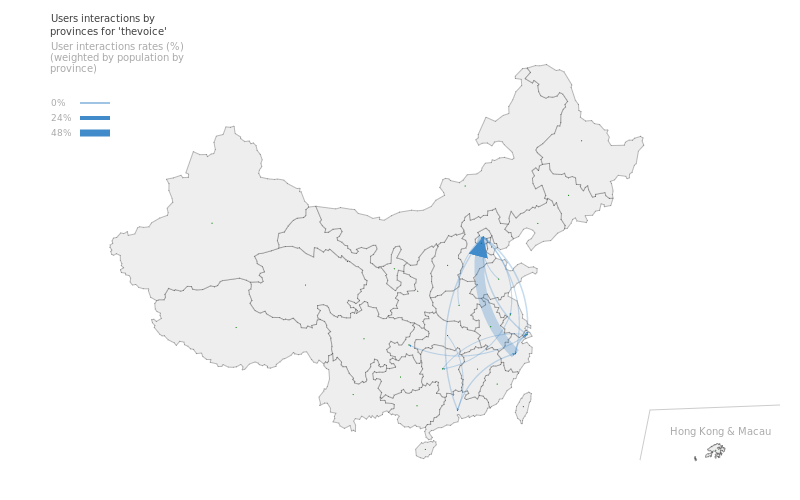
\includegraphics[width=4.6606in,height=2.913in]{figures/chap4/chapitre4-img19.png}
  \caption{
    The Voice: Interaction des utilisateurs par province entre le 9 et le 29 Juillet 2012
  }
\end{figure}

Dans le cas de \textit{The Voice}, nous pouvons voir que
l{\textquoteright}interaction est structur\'e autour
d{\textquoteright}un axe fort entre la province de Zhejiang et P\'ekin.
Cela s{\textquoteright}explique assez simplement par le fait que
l{\textquoteright}\'emission est diffus\'e par Zhejiang T\'el\'evision
dont le compte officiel joue un r\^ole important dans la diffusion et
la promotion de la discussion.
\begin{figure}
    \centering
    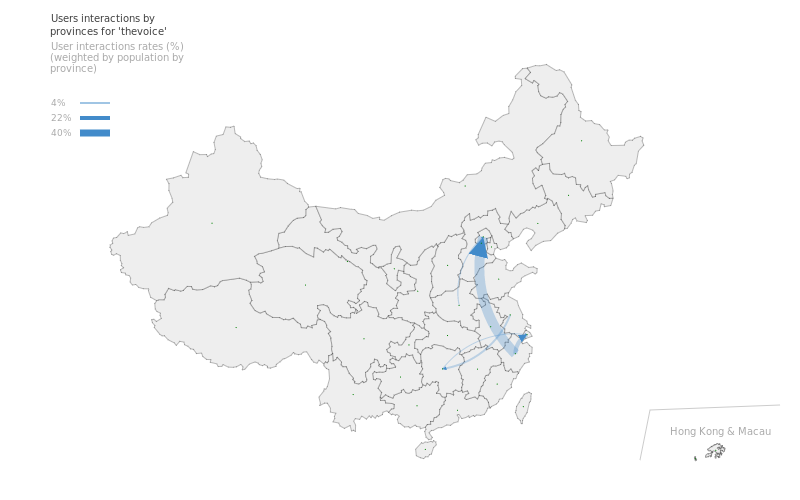
\includegraphics[width=4.3858in,height=2.7413in]{figures/chap4/chapitre4-img20.png}
    
  \caption{
    Figure (1)The Voice: Interaction des utilisateurs par province entre le 16 et le 17 Juillet 2012
  }
\end{figure}

En isolant uniquement le soir de la premi\`ere diffusion, on voit que
cette structure s{\textquoteright}accentue encore davantage et que les
interactions se structurent entre le Zhejiang P\'ekin et Shanghai avec
quelques autres axes plus minoritaires.

\begin{figure}
    \centering
    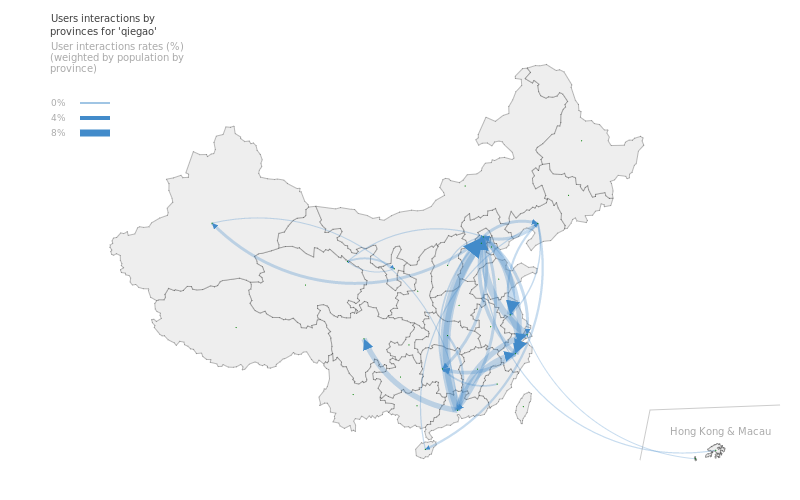
\includegraphics[width=5.7059in,height=3.5661in]{figures/chap4/chapitre4-img21.png}
  \caption{
    Qiegao: Interaction des utilisateurs par province entre le 19 Novembre et le 15 D\'ecembre 2012
  }
\end{figure}


A l{\textquoteright}inverse, nous voyons que pour \textit{Qiegao} les
patterns semblent beaucoup plus diversifi\'es. Guangzhou joue un r\^ole
de diffuseur important et beaucoup d{\textquoteright}informations
converge vers Shanghai et P\'ekin. De nombreuses conversations se
d\'eroulent \'egalement dans l{\textquoteright}ouest de la Chine. En
effet, la discussion concerne ici les peuples Uyghur et on constate que
les habitants du Xinjiang participent davantage \`a la conversation que
dans d{\textquoteright}autres m\`emes. 

\begin{figure}
    \centering
    \subfloat[Jour 1: 3 D\'ecembre 2012]{
      \label{fig:edge-a}
      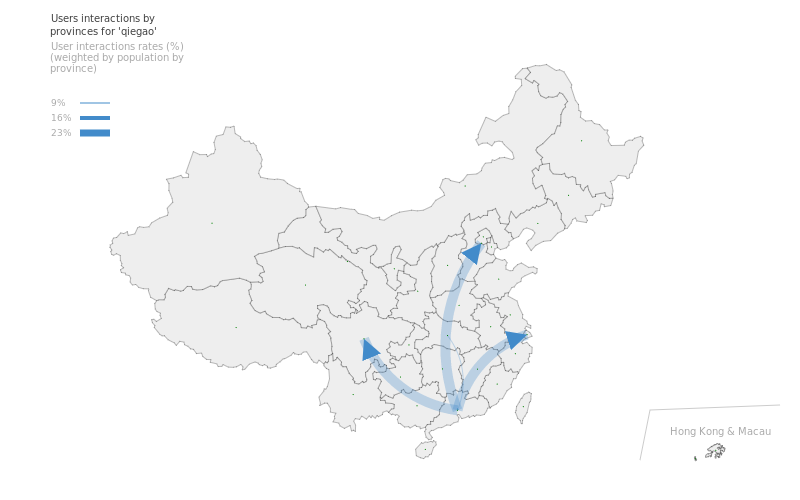
\includegraphics[width=2.9579in,height=1.8488in]{figures/chap4/chapitre4-img22.png}
    }
    \subfloat[Jour 2-3: 4-5 D\'ecembre 2012]{
      \label{fig:edge-a}
      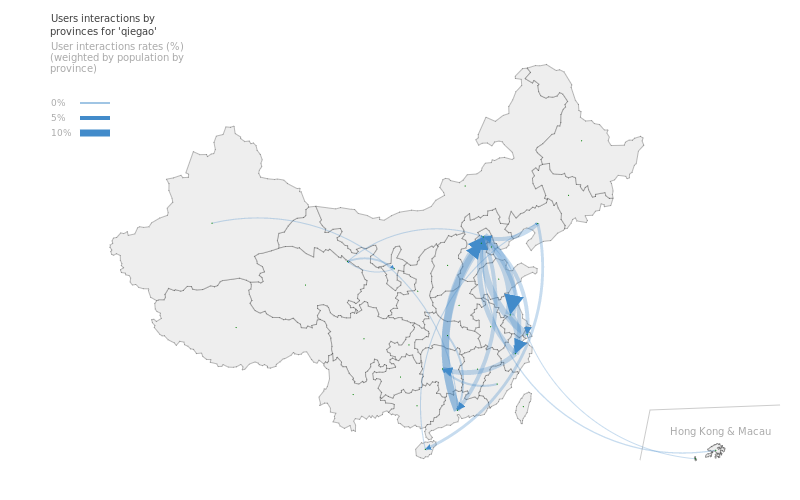
\includegraphics[width=2.8039in,height=1.7531in]{figures/chap4/chapitre4-img23.png}    }
    \subfloat[Jour 4-6: 6-8 D\'ecembre 2012]{
      \label{fig:edge-a}
      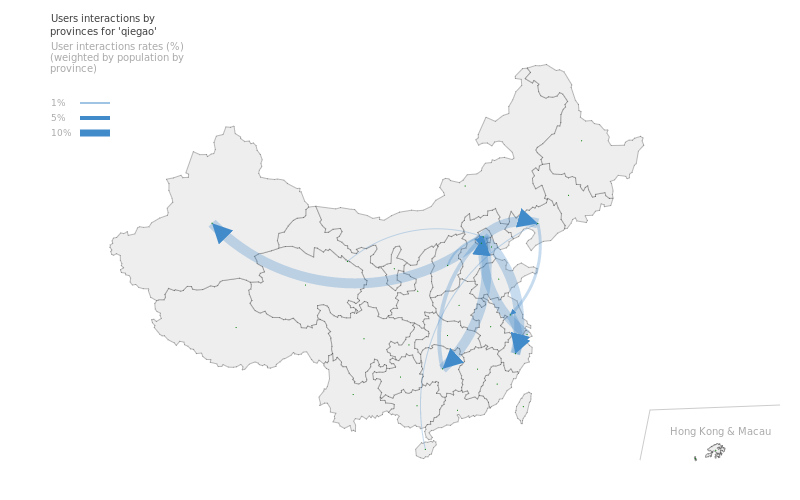
\includegraphics[width=2.8886in,height=1.8059in]{figures/chap4/chapitre4-img24.png}
    }
    \subfloat[Jour 7+: 9-16 D\'ecembre 2012]{
      \label{fig:edge-a}
      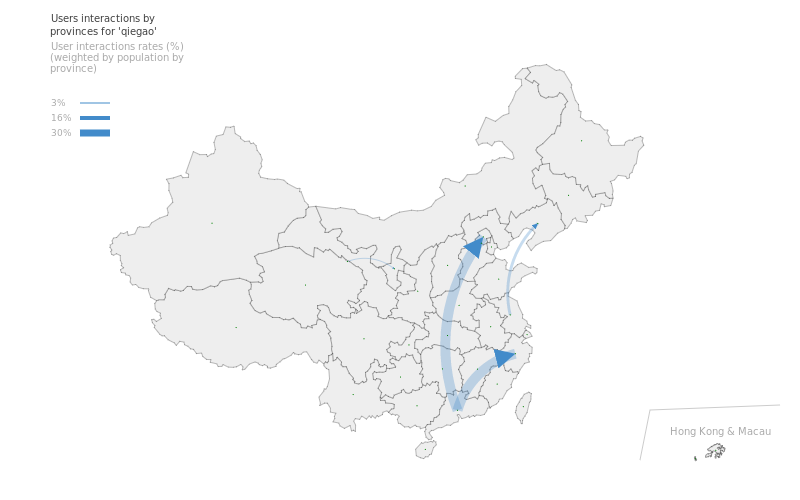
\includegraphics[width=2.8724in,height=1.7961in]{figures/chap4/chapitre4-img25.png}   
  
    }
    
  \caption{
    Qiegao: Interaction des utilisateurs par province
  }
\end{figure}

  


En consid\'erant l{\textquoteright}\'evolution du m\`eme dans le temps,
nous voyons qu{\textquoteright}il \'emane d{\textquoteright}abord de
Canton, puis se diffuse \`a P\'ekin et Shanghai qui semble jouer un
r\^ole d{\textquoteright}amplificateur en le diffusant plus largement,
notamment vers l{\textquoteright}Ouest. 



\begin{figure}
    \centering
    
    \subfloat[Jour 1: 22 Novembre 2012]{
      \label{fig:edge-a}
    
    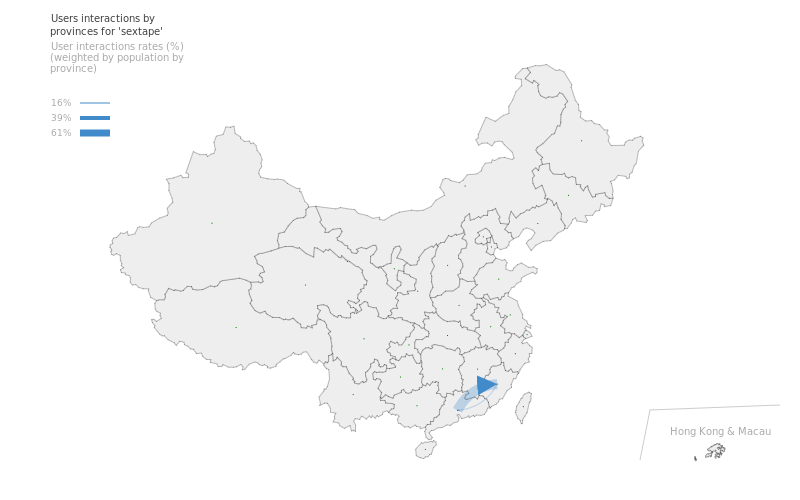
\includegraphics[width=1.9587in,height=1.2248in]{figures/chap4/chapitre4-img26.png}
    }
    \subfloat[Jour 2-5: 23-25 Novembre 2012]{
      \label{fig:edge-a}
      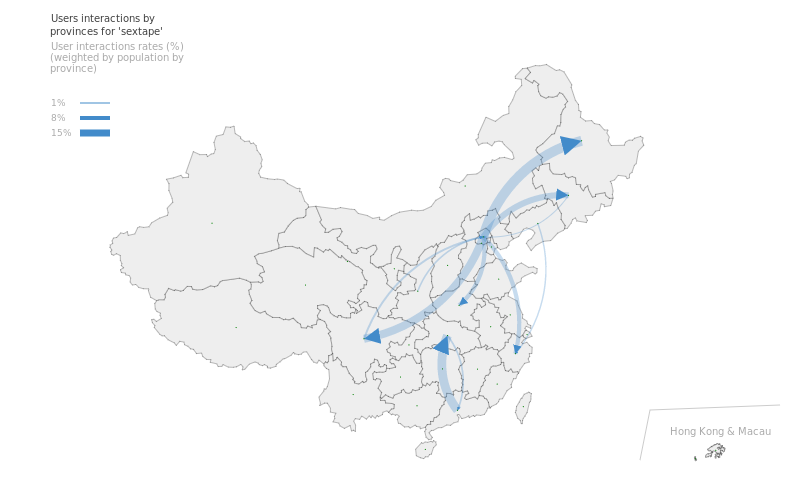
\includegraphics[width=1.9386in,height=1.2114in]{figures/chap4/chapitre4-img27.png}
    }
    \subfloat[Jour 5+: 26 Nov-15 D\'ec 2012]{
      \label{fig:edge-a}
      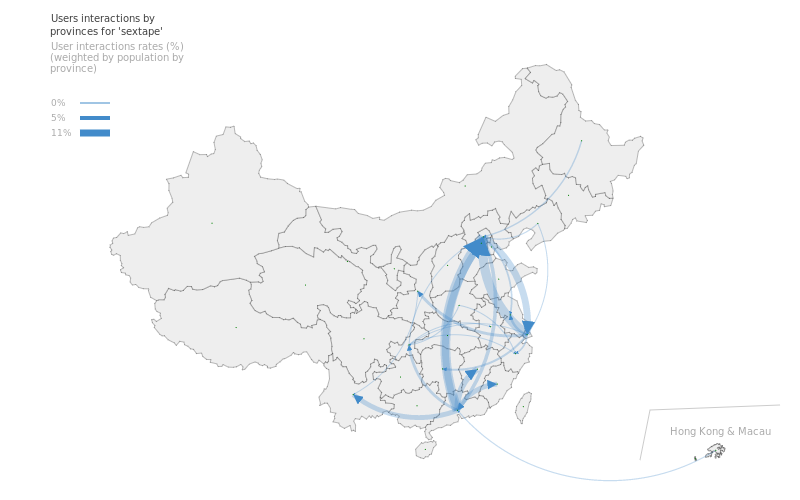
\includegraphics[width=2.0012in,height=1.2512in]{figures/chap4/chapitre4-img28.png}
    }    
  \caption{
    Sextape: Interaction des utilisateurs par province
  }
\end{figure}

\begin{figure}
    \subfloat[Jour 1-3 : 26-28 Aout 2012 ]{
      \label{fig:edge-a}
      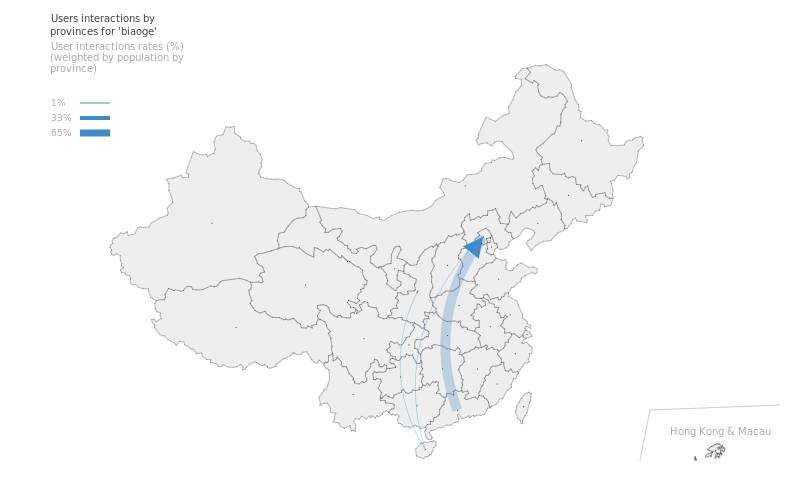
\includegraphics[width=1.9004in,height=1.1878in]{figures/chap4/chapitre4-img29.png} 
    }
    \subfloat[Jour 4-5 : 29-30 Aout 2012 ]{
      \label{fig:edge-a}
      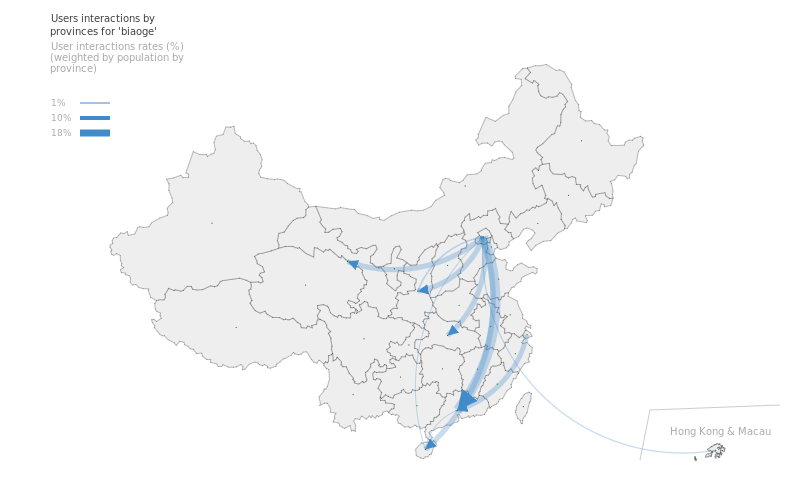
\includegraphics[width=1.9004in,height=1.1878in]{figures/chap4/chapitre4-img30.png} 
    }
    \subfloat[Jour 5+ : 1-3 Septembre2012]{
      \label{fig:edge-a}
      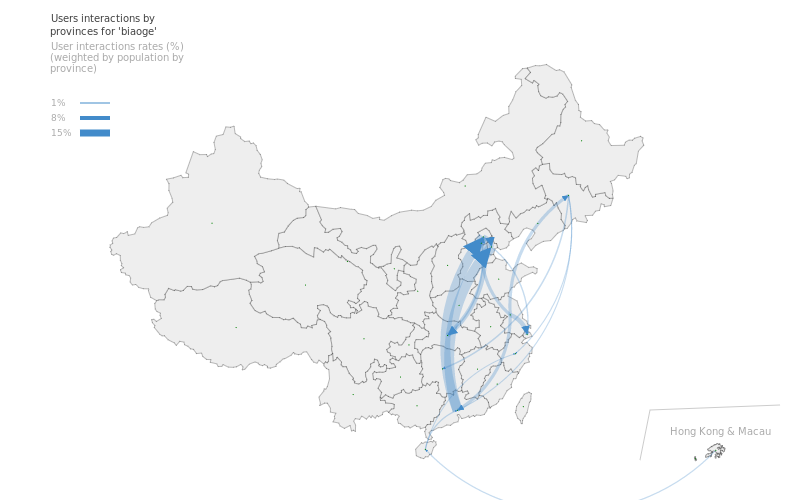
\includegraphics[width=1.9004in,height=1.1878in]{figures/chap4/chapitre4-img31.png} 
    }
  \caption{
    Fig (3) Biaoge: Interaction des utilisateurs par province
  }
\end{figure}

On retrouve \'egalement ce pattern pour d{\textquoteright}autres faits
de soci\'et\'e comme \textit{sextape} ou \textit{biaoge. }Cela illustre
bien le r\^ole particulier des m\'edias du sud de la Chine et plus
sp\'ecialement celui de Guangzhou. Avec une plus grande libert\'e de
ton et une plus grande latitude dans leur propos, les m\'edias
cantonais sont bien souvent instigateurs d{\textquoteright}affaires
importantes alors que les m\'edias p\'ekinois, plus conservateurs joue
plut\^ot un r\^ole de diffuseur. 

% \begin{figure}
%   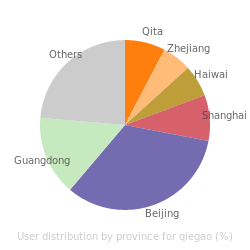
\includegraphics[width=0.0012in,height=0.0012in]{figures/chap4/chapitre4-img32.png}
% \end{figure}

\begin{figure}
    \subfloat[ Qiegao]{
      \label{fig:edge-a}
      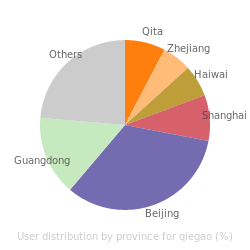
\includegraphics[width=1.9016in,height=1.9016in]{figures/chap4/chapitre4-img33.png}
    }
    \subfloat[Sextape]{
      \label{fig:edge-a}
      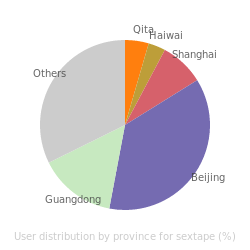
\includegraphics[width=1.9016in,height=1.9016in]{figures/chap4/chapitre4-img34.png}
    }
    \subfloat[Biaoge]{
      \label{fig:edge-a}
      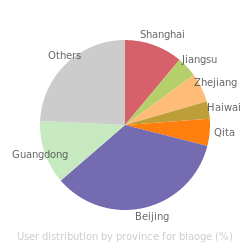
\includegraphics[width=1.9016in,height=1.9016in]{figures/chap4/chapitre4-img35.png}
    }
  \caption{
    R\'epartition des utilisateurs par province (en \% du total)
  }
\end{figure}



En observant la r\'epartition des utilisateurs par province pour chacun
de ces trois m\`emes, on remarque que Beijing, Canton, Shanghai ont une
place importante, ainsi que les personnes situ\'ees \`a
l{\textquoteright}\'etranger (Haiwai) et le Zhejiang. N\'eanmoins, le
reste des provinces (repr\'esent\'es ici par
{\textquotedblleft}Others{\textquotedblright} en gris) constitue une
part importante des \'echanges.

\begin{figure}
    \centering

    \subfloat[Jour 1: 12 Octobre 2012]{
      \label{fig:time-moyan1}
      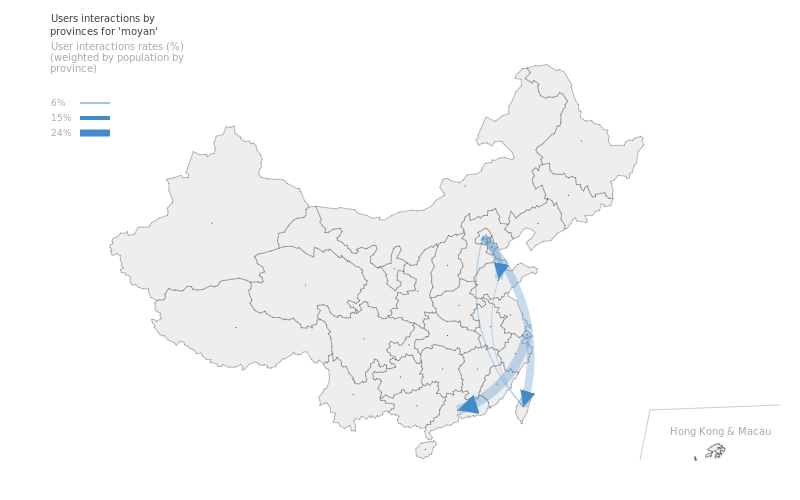
\includegraphics[width=1.9004in,height=1.1878in]{figures/chap4/chapitre4-img36.png}
    }
     
    \subfloat[Jour 2: 13 Octobre 2012]{
      \label{fig:time-moyan2}
      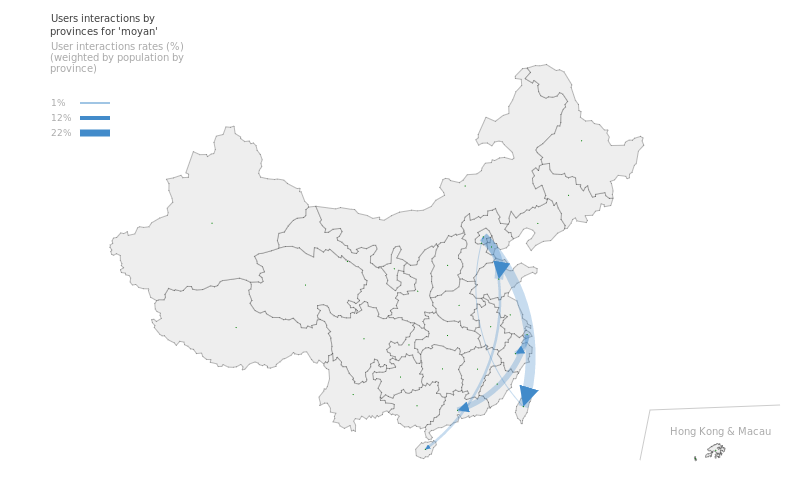
\includegraphics[width=1.9004in,height=1.1878in]{figures/chap4/chapitre4-img37.png}
    }

    \subfloat[Jour 3+: 14-21 Octobre 2012]{
      \label{fig:time-moyan3}
      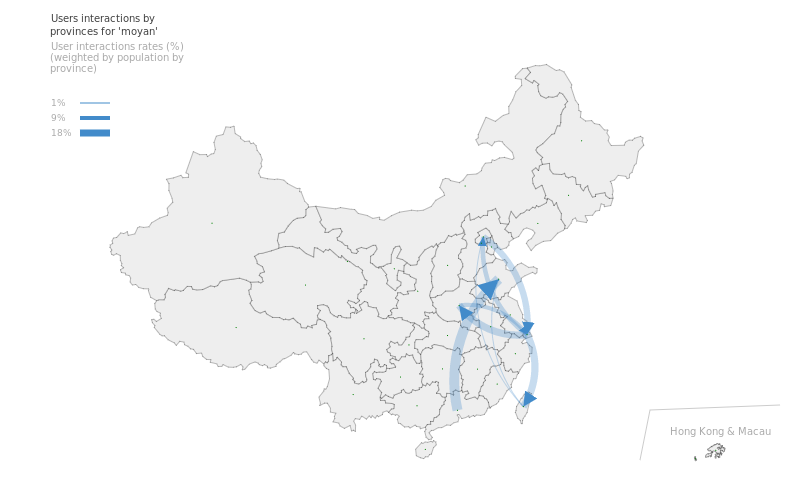
\includegraphics[width=1.9004in,height=1.1878in]{figures/chap4/chapitre4-img38.png}
    }

    \caption{
        Moyan : Interaction des utilisateurs par province   
    }

\end{figure}


Dans le cas de nouvelles plus officielles comme pour \textit{Moyan
}notamment, nous pouvons voir que l{\textquoteright}information
s{\textquoteright}origine g\'en\'eralement de P\'ekin et se diffuse
vers le sud et le centre. 

\begin{figure}
    \centering
    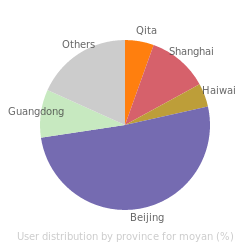
\includegraphics[width=2.6043in,height=2.6043in]{figures/chap4/chapitre4-img39.png}
  \caption{
    R\'epartition des utilisateurs par province (en \% du total)\\
  }
\end{figure}


La composition des utilisateurs montre bien que les d\'ebats sont tr\`es
largement domin\'es par P\'ekin avec plus de 50\% de
l{\textquoteright}activit\'e impliquant au moins un utilisateur
identifi\'e \`a P\'ekin.

Dans le cas des m\`emes absurdistes et comiques, il est int\'eressant de
constater qu{\textquoteright}ils ne se construisent pas
n\'ecessairement sur les patterns que nous avons pu observ\'es
auparavant.

\begin{figure}
    \centering

    \subfloat[dufu]{
      \label{fig:time-moyan1}
      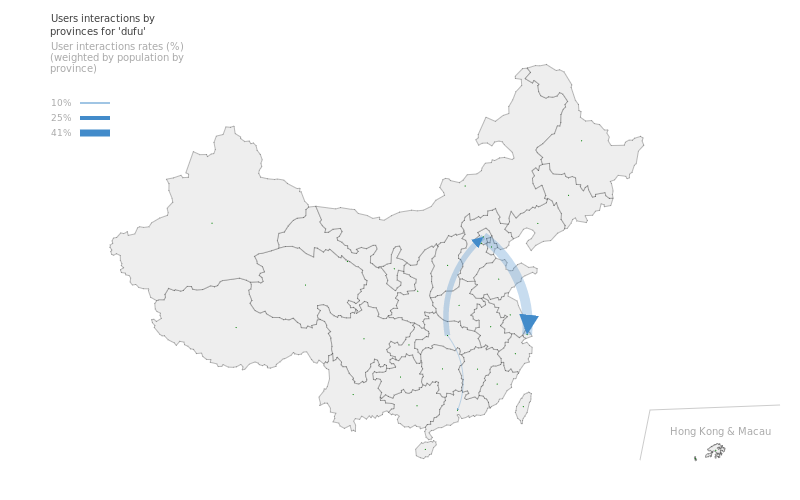
\includegraphics[width=2.9252in,height=1.828in]{figures/chap4/chapitre4-img40.png}
    }
     
    \subfloat[yuanfang]{
      \label{fig:time-moyan2}
      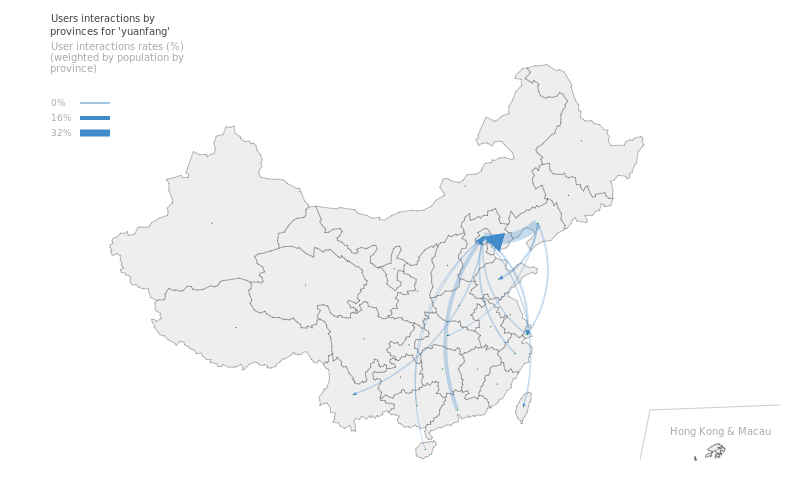
\includegraphics[width=2.9252in,height=1.828in]{figures/chap4/chapitre4-img41.png}
    }

    \caption{
        Interaction des utilisateurs par province
    }

\end{figure}


On voit notamment que le m\`eme \textit{dufu }d\'ebute dans la r\'egion
du Hubei alors que le Liaoning joue un r\^ole cl\'e dans la diffusion
de \textit{yuanfang.} 
\begin{figure}
    \centering

    \subfloat[(Dufu) Jour 1-2 : 23 au 25 Mars 2012 ]{
      \label{fig:time-moyan1}
      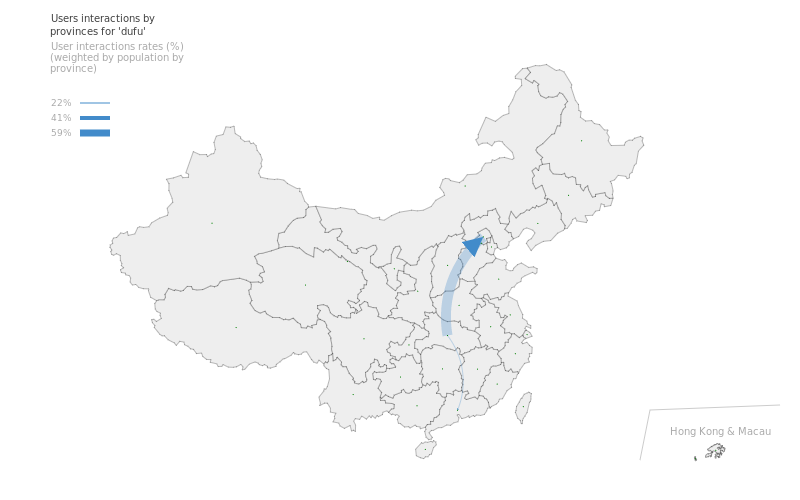
\includegraphics[width=2.9252in,height=1.828in]{figures/chap4/chapitre4-img42.png}
    }
     
    \subfloat[(Dufu) Jour 3+ : 25 Mars au 15 Avril]{
      \label{fig:time-moyan2}
      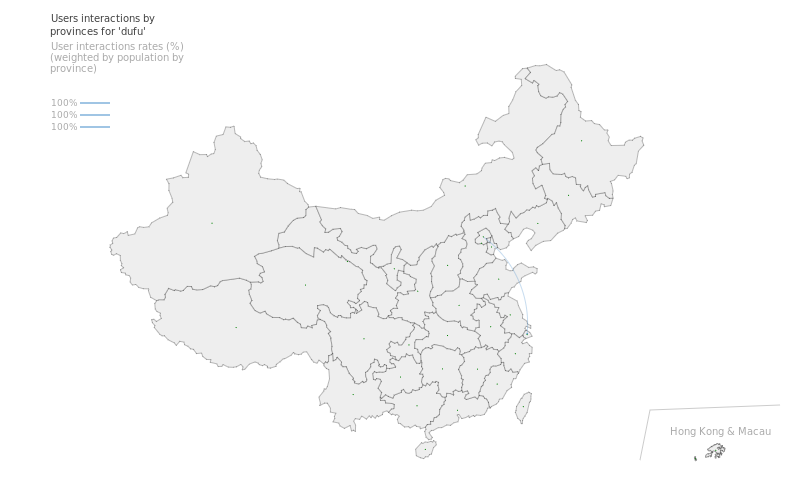
\includegraphics[width=2.9713in,height=1.8571in]{figures/chap4/chapitre4-img43.png}
    }
    \subfloat[(Yuanfang) Jour 1-2: 15 au 17 Octobre 2012]{
      \label{fig:time-moyan2}
      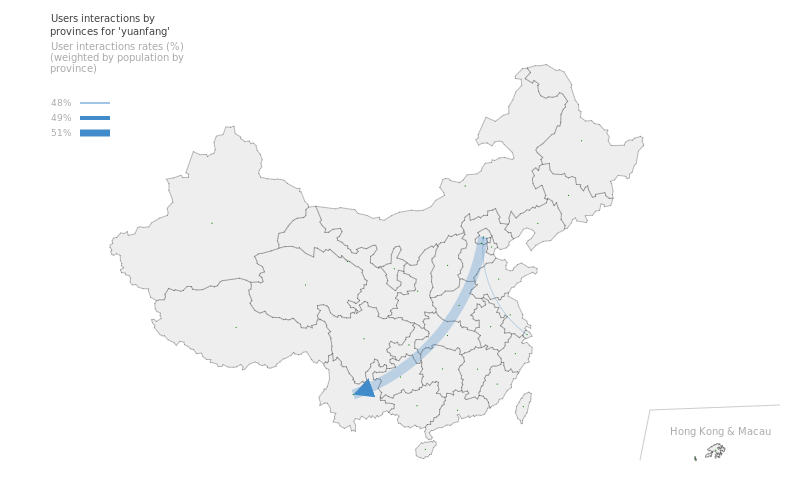
\includegraphics[width=2.9252in,height=1.828in]{figures/chap4/chapitre4-img44.png}
    }
    \subfloat[(Yuanfang) Jour 3+: 18 Oct au 16 D\'ecembre 2012]{
      \label{fig:time-moyan2}
      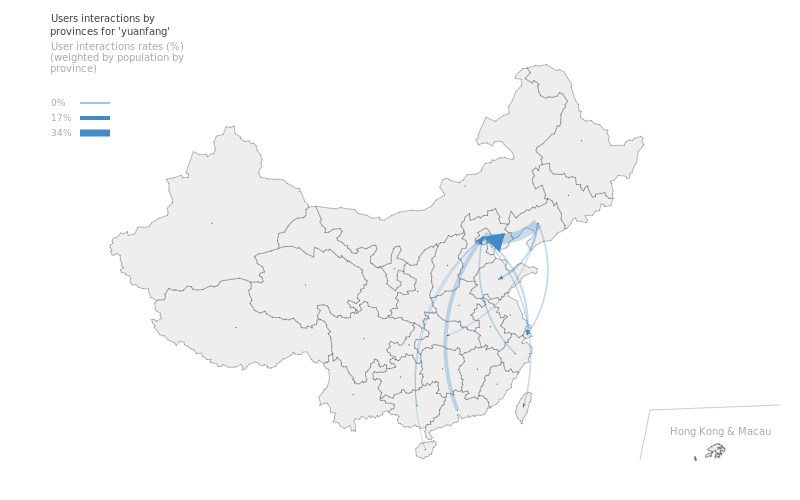
\includegraphics[width=2.9252in,height=1.828in]{figures/chap4/chapitre4-img45.png}
    }
    
    \caption{
        Interaction des utilisateurs par province
    }

\end{figure}



En consid\'erant les graphes de temps, on remarque \'egalement que si
P\'ekin est bien pr\'esent, les \'echanges des premiers jours se font
avec le Hubei et le Yunnan, deux provinces typiquement peu actives. 

\begin{figure}
    \centering

    \subfloat[dufu]{
      \label{fig:time-moyan1}
      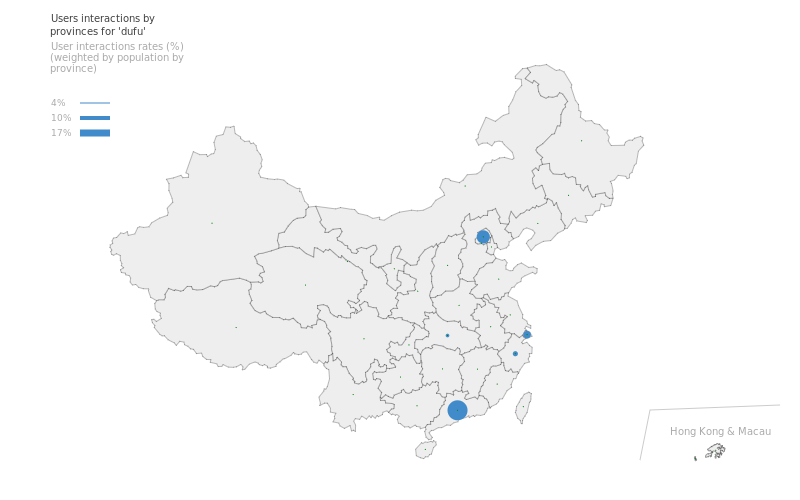
\includegraphics[width=2.9252in,height=1.828in]{figures/chap4/chapitre4-img46.png}
    }
     
    \subfloat[yuanfang]{
      \label{fig:time-moyan2}
      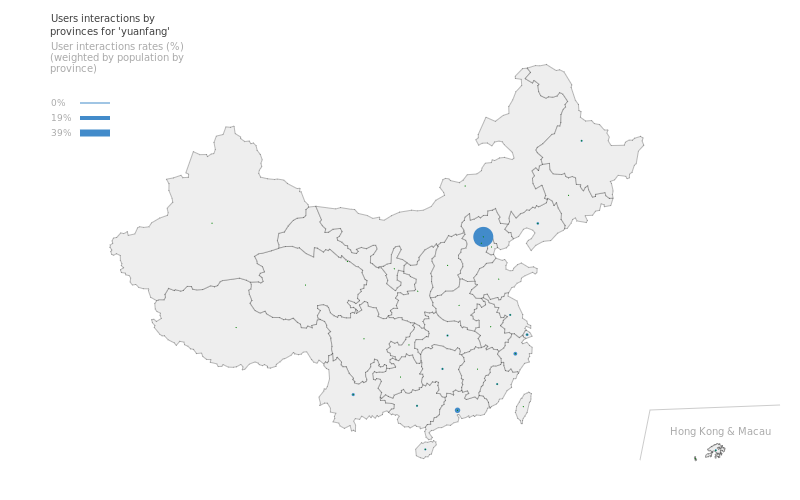
\includegraphics[width=2.9252in,height=1.828in]{figures/chap4/chapitre4-img47.png}
    }

    \caption{
        Interaction entre utilisateurs de la m\^eme province
    }

\end{figure}

En s{\textquoteright}int\'eressant aux \'echanges qui se d\'eroulent au
sein de chaque province (d{\textquoteright}un utilisateur situ\'e dans
une province vers un autre utilisateur situ\'e dans la meme province),
nous constatons que les \'echanges internes sont \'egalement importants
au sein des villes principales (Canton, P\'ekin et Shanghai) mais de
nombreuses villes prennent aussi par \`a la discussion. 


\begin{figure}
    \centering

    \subfloat[dufu]{
      \label{fig:time-moyan1}
      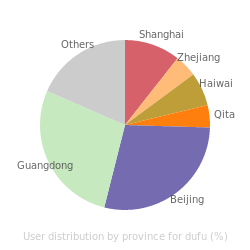
\includegraphics[width=2.6043in,height=2.6043in]{figures/chap4/chapitre4-img48.png}
    }
     
    \subfloat[yuanfang]{
      \label{fig:time-moyan2}
      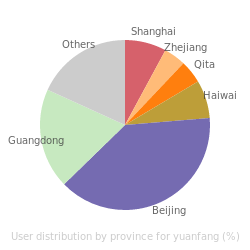
\includegraphics[width=2.6043in,height=2.6043in]{figures/chap4/chapitre4-img49.png}
    }

    \caption{
        R\'epartition des utilisateurs par province (en \% du total)
    }

\end{figure}


\subsubsection{4122. Communaut\'es, clusters et groupes de provinces}
Un r\'ecent article du d\'epartement d{\textquoteright}urbanisme de
l{\textquoteright}Universit\'e de Nanjing (Zhen \&al., 2014) analyse
les relations entre le r\'eseau urbain et le r\'eseau
qu{\textquoteright}il est possible d{\textquoteright}inf\'erer au sein
des relations friends/followers entre les utilisateurs sur Sina Weibo .
Il y est notamment montr\'e que le r\'eseau des relations entre
utilisateurs vient renforcer la hi\'erarchie classique du syst\`eme
urbain en acc\'el\'erant l{\textquoteright}agglom\'eration selon des
mod\`eles spatiaux pr\'e-existants comme celui le pattern des
\textit{{\textquotedblleft}Three majors }\textit{and four
smalls{\textquotedblright} }montrant aussi une diff\'erence tr\`es
marqu\'e entre l{\textquoteright}Ouest et l{\textquoteright}Est.


\begin{figure}
    \centering
    
    \begin{description}
    \item Three Majors
      \begin{enumerate}
      \item Pearl River Delta (Guangzhou, Shenzhen)
      \item Beijing-Tianjin-Hebei region (Beijing)
      \item the Yangtze River Delta (Shanghai, Hangzhou, Nanjing)
      \end{enumerate}

    \item Four Smalls
      \begin{enumerate}
      \item Chengdu-Chongqing region (Chengdu, Chongqing)
      \item Hercynian region (Fuzhou, Xiamen)
      \item Wuhan (central) region (Wuhan, Changsha)
      \item Northeast China (Shenyang, Harbin, Changchun)
      \end{enumerate}

    \end{description}

   \caption{
      Le mod\`ele urbain chinois du Three majors and four smalls d{\textquoteright}apr\`es \cite{Zhen2014}
    }
\end{figure}


Nous avons donc d\'ecid\'e de comparer ces r\'esultats obtenus depuis le
r\'eseau des followers sur Sina Weibo avec les ph\'enom\`enes
observ\'es lors de la diffusion de contenus. En effet, si on peut
affirmer que le r\'eseau
{\textquotedblleft}d{\textquoteright}amis{\textquotedblright} structure
les canaux de diffusion de Sina Weibo, ces canaux ne sont pas
n\'ecessairement sujets \`a une utilisation fr\'equente et donc \`a
l{\textquoteright}actualisation de ces structures.


Afin d{\textquoteright}observer les patterns form\'es par les
diff\'erents m\`emes en se diffusant, nous continuons
d{\textquoteright}utiliser le r\'eseau des interactions entre provinces
des utilisateurs. Afin de d\'etecter les communaut\'es de discussion et
identifier les provinces ayant interagit le plus ensemble dans chaque
cas, nous soumettons le r\'eseau d{\textquoteright}interactions \`a un
algorithme de Louvain (Blondel \& al., 2008). Sur les cartes, les
couleurs repr\'esentent les diff\'erentes communaut\'es calcul\'ees
depuis le r\'eseau d{\textquoteright}interactions.

\begin{figure}
    \centering

    \subfloat[sextape]{
      \label{fig:time-moyan1}
      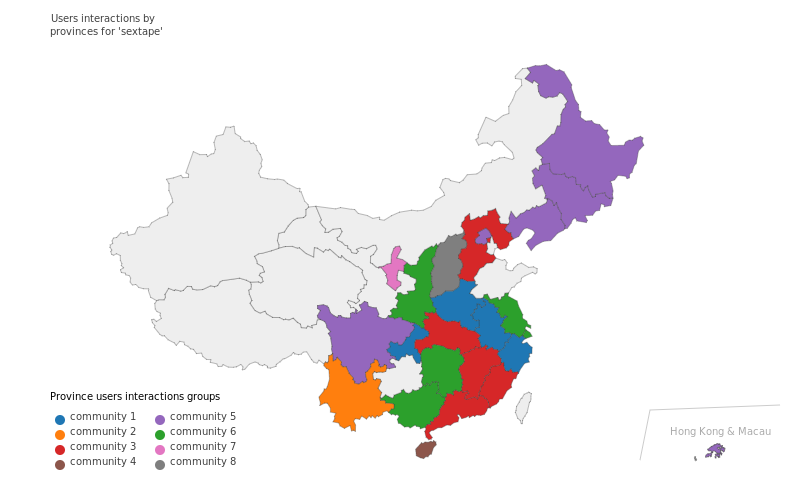
\includegraphics[width=3.198in,height=2.0004in]{figures/chap4/chapitre4-img50.png}
    }
     
    \subfloat[TheVoice]{
      \label{fig:time-moyan2}
      \includegraphics[width=3.3024in,height=2.063in]{figures/chap4/chapitre4-img51.png}
    } 
    \subfloat[Qiegao]{
      \label{fig:time-moyan2}
      \includegraphics[width=3.1878in,height=1.9795in]{figures/chap4/chapitre4-img52.png}
    } 
    \subfloat[Dufu]{
      \label{fig:time-moyan2}
      \includegraphics[width=3.5315in,height=2.2087in]{figures/chap4/chapitre4-img53.png}
    }

    \caption{
        Communaut\'e de provinces dessin\'ees par les \'echanges entre utilisateurs autour de chaque m\`eme 
    }

\end{figure}


A la premi\`ere lecture de ces cartes, nous constatons en effet que les
provinces de l{\textquoteright}Ouest sont nettement moins engag\'ees
que celles de la moiti\'e Est de la Chine. Ce fait refl\`ete la
population utilisateurs de Weibo concentr\'es en majorit\'e dans les
grandes villes en d\'eveloppement de la c\^ote et du centre (Fu \&
Chau, 2013). 

Le m\`eme absurdiste \textit{dufu }poss\`ede une diffusion plus
concentr\'ee alors que les discussions politiques semblent regrouper
des utilisateurs d{\textquoteright}origines plus diverses. Nous
remarquons \'egalement que Taiwan est absente des discussions plus en
lien avec la politique et la soci\'et\'e de Chine continentale, alors
qu{\textquoteright}elle est bien pr\'esente dans le cas des m\`emes
absurdistes et de l{\textquoteright}\'emission de loisir. 

Devant la diversit\'e de contenus propos\'es par ces cartes, peu de
pattern sont d\'ecelables a priori et la circulation des contenus ne
semble pas suivre les patterns observ\'es dans les relations friends /
followers.


Ces premi\`eres observations nous montre qu{\textquoteright}il est
possible de mieux comprendre les logiques et dynamiques de diffusion
des contenus, mais il est n\'eanmoins plus p\'erilleux de consid\'erer
les usages du r\'eseau pour en tirer des conclusions sur les dynamiques
g\'eographiques d{\textquoteright}ensemble d{\textquoteright}un
territoire. De plus, nous ne disposons que de tr\`es peu
d{\textquotesingle}aspects
{\textquotedbl}g\'eo-localis\'es{\textquotedbl} dans ces donn\'ees (pas
de g\'eotag sur chaque message \`a proprement parler) et nous savons
que la province d{\textquoteright}origine du profil ne peut \^etre
consid\'er\'e comme une source absolument fiable. Les utilisateurs sont
en effet libres de la remplir selon leur bon vouloir. De plus, cette
information est \'ecrite une fois pour toute et n{\textquoteright}ai
pas n\'ecessairement mise \`a jour lors des d\'eplacements ou m\^eme
d\'em\'enagements des utilisateurs.


\subsubsection{Dimensions g\'eographiques des graphes socio-s\'emantiques}
Face \`a ces diverses r\'eserves, nous voyons qu{\textquoteright}il est
important de recentrer l{\textquoteright}\'etude sur les modes de
diffusion et leurs dimensions socio-s\'emantiques. Afin de continuer
notre exploration des dynamiques conversationnelles entourant les
\'echanges en ligne, nous allons donc nous int\'eresser au croisement
de ces diff\'erentes dimensions en consid\'erant les corr\'elations
entre les mots, les utilisateurs et les provinces \`a diff\'erents
niveaux.


Tout d{\textquoteright}abord, nous nous proposons
d{\textquoteright}observer la distribution des provinces
d{\textquoteright}origine des communaut\'es
d{\textquoteright}utilisateurs les plus importantes. En s\'electionnant
les communaut\'es les plus centrales pour chaque graphe, nous pouvons
mieux comprendre comment se r\'epartissent les
{\textquotedblleft}influenceurs{\textquotedblright} sur le territoire
pour chacun des m\`emes choisis ici.

\begin{figure}
    \centering

    \subfloat[sextape]{
      \label{fig:time-moyan1}
      \includegraphics[width=5.9996in,height=2.5004in]{figures/chap4/chapitre4-img54.png}
    }
     
    \subfloat[biaoge]{
      \label{fig:time-moyan2}
      \includegraphics[width=5.9996in,height=2.5004in]{figures/chap4/chapitre4-img55.png}
    } 
   

    \caption{
        % Communaut\'e de provinces dessin\'ees par les \'echanges entre utilisateurs autour de chaque m\`eme 
    }

\end{figure}

 

Les communaut\'es form\'ees lors de la discussion autour des m\`emes \`a
teneur plus politique pr\'esentent une grande diversit\'e de
provenances. On voit dans le cas de \textit{biaoge} et \textit{sextape
}que de nombreuses provinces sont repr\'esent\'ees. 


\begin{figure}
    \centering

    \includegraphics[width=5.9996in,height=2.5004in]{figures/chap4/chapitre4-img56.png}
   

    \caption{
        % Communaut\'e de provinces dessin\'ees par les \'echanges entre utilisateurs autour de chaque m\`eme 
        The Voice
    }

\end{figure}




A l{\textquoteright}inverse, les communaut\'es
d{\textquoteright}utilisateurs les plus impliqu\'ees dans \textit{The
Voice }ou \textit{Moyan} sont pour la plupart localis\'ees \`a Beijing.
Par rapport \`a la cartographie pr\'ec\'edente qui montrait les
relations fortes avec le Zhejiang pour \textit{The Voice}, nous voyons
ici que la province est tr\`es faiblement repr\'esent\'ee dans les
communaut\'es majoritaires.


  \begin{figure}
    \centering

   \includegraphics[width=5.9996in,height=2.5004in]{figures/chap4/chapitre4-img57.png}
   

    \caption{
        % Communaut\'e de provinces dessin\'ees par les \'echanges entre utilisateurs autour de chaque m\`eme 
        Moyan
    }

\end{figure}


Le m\`eme \textit{dufu }montre quant \`a lui un patterns diff\'erents
o\`u les communaut\'es sont plus organis\'ees plus r\'egionalement,
avec moins de diversit\'e d{\textquoteright}origine des utilisateurs
engag\'es dans les discussions.


\begin{figure}
    \centering

   \includegraphics[width=5.9996in,height=2.5004in]{figures/chap4/chapitre4-img58.png}
   

    \caption{
        % Communaut\'e de provinces dessin\'ees par les \'echanges entre utilisateurs autour de chaque m\`eme 
        Dufu
    }

\end{figure}


 


Une dimension importante du m\`eme absurdiste semble \^etre
l{\textquoteright}organisation des conversations en communaut\'es
plut\^ot local (utilisateurs de m\^eme provinces). Une premi\`ere
analyse des communaut\'es les plus centrales dans le graphe de
\textit{yuanfang }ne nous permet de retrouver ce pattern. Pourtant, en
nous int\'eressant aux communaut\'es de seconde et troisi\`eme
importances, nous voyons que la plupart se constituent autour de 1 ou 2
provinces seulement. 


Pour continuer notre exploration de l{\textquoteright}existence
g\'eographique des relations socio-s\'emantiques dans nos m\`emes, nous
allons maintenant nous int\'eresser \`a une seconde dimension qui est
celle de la distribution des mots par province. Nous s\'electionnons
pour chaque m\`eme les mots les plus centraux du graphe s\'emantique et
d\'ecomposons leur usage afin de comprendre la diversit\'e ou
l{\textquoteright}unicit\'e de l{\textquoteright}origine des
utilisateurs.


\begin{figure}
    \centering
    \includegraphics[width=6.0087in,height=3.3386in]{figures/chap4/chapitre4-img59.png}
    \caption{
      biaoge : distribution des citations par provinces pour le mot wan signifiant 10000, une quantit\'e ici quantit\'e d{\textquoteright}argent pour une montre.
    }
\end{figure}
 



\begin{figure}
    \centering
    \subfloat[Légende 1]{
      \label{fig:edge-a}
      \includegraphics[width=6.0087in,height=3.3386in]{figures/chap4/chapitre4-img60.png}
    }
  \caption{
     biaoge : distribution des citations par provinces pour le mot biao (montre)
  }
\end{figure}


Dans le cas du m\`eme biaoge, nous voyons que les mots principaux
portent une forte diversit\'e et confirme l{\textquoteright}hypoth\`ese
d{\textquoteright}une diffusion g\'eographique plus large de la
discussion.


\begin{figure}
    \centering

    \subfloat[\textit{zhen}, signifiant {\textquotedblleft}vrai{\textquotedblright}]{
      \label{fig:edge-a}
      \includegraphics[width=6.0087in,height=3.3386in]{figures/chap4/chapitre4-img61.png}
    }
    \subfloat[\textit{chang}, signifiant {\textquotedblleft}chanter{\textquotedblright}]{
      \label{fig:edge-a}
      \includegraphics[width=6.0087in,height=3.3386in]{figures/chap4/chapitre4-img62.png}
    }
    \subfloat[\textit{shengyin}, signifiant "la voix"]{
      \label{fig:edge-a}
      \includegraphics[width=6.0087in,height=3.3386in]{figures/chap4/chapitre4-img63.png}
    }

  \caption{
    The Voice : distribution des citations de mots par provinces 
  }
\end{figure}


A l{\textquoteright}inverse, les mots-cl\'es de \textit{The Voice} sont
nettement domin\'es par des communaut\'es d{\textquoteright}utilisateurs de P\'ekin ou du Zhejiang qui semble r\'eellement fixer les termes de la discussion.

\begin{figure}
    \centering
    \subfloat{  
      \includegraphics[width=6.0087in,height=3.3386in]{figures/chap4/chapitre4-img64.png}
    }
    \subfloat{  
      \includegraphics[width=6.0087in,height=3.3386in]{figures/chap4/chapitre4-img65.png}
    }
    \subfloat{  
      \includegraphics[width=6.0087in,height=3.3386in]{figures/chap4/chapitre4-img66.png}
    }

    \caption{
      Légende ???
    }
\end{figure}

Dans le cas de dufu, les trois mots les plus importants
\textit{dufu}, \textit{zuijin} et \textit{mang} qui forme la
phrase-m\`eme \textit{dufu est tr\`es occup\'e
r\'ecemment }sont tous tr\`es fortement reli\'e \`a
la r\'egion de Canton. Cette information, pas forc\'ement pro\'eminente
dans les analyses pr\'ec\'edentes, montrent que le d\'eveloppement de
ce m\`eme est largement le fait d{\textquoteright}utilisateurs de la
r\'egion de Canton.